% Options for packages loaded elsewhere
\PassOptionsToPackage{unicode}{hyperref}
\PassOptionsToPackage{hyphens}{url}
%
\documentclass[
  man,floatsintext]{apa6}
\usepackage{amsmath,amssymb}
\usepackage{iftex}
\ifPDFTeX
  \usepackage[T1]{fontenc}
  \usepackage[utf8]{inputenc}
  \usepackage{textcomp} % provide euro and other symbols
\else % if luatex or xetex
  \usepackage{unicode-math} % this also loads fontspec
  \defaultfontfeatures{Scale=MatchLowercase}
  \defaultfontfeatures[\rmfamily]{Ligatures=TeX,Scale=1}
\fi
\usepackage{lmodern}
\ifPDFTeX\else
  % xetex/luatex font selection
\fi
% Use upquote if available, for straight quotes in verbatim environments
\IfFileExists{upquote.sty}{\usepackage{upquote}}{}
\IfFileExists{microtype.sty}{% use microtype if available
  \usepackage[]{microtype}
  \UseMicrotypeSet[protrusion]{basicmath} % disable protrusion for tt fonts
}{}
\makeatletter
\@ifundefined{KOMAClassName}{% if non-KOMA class
  \IfFileExists{parskip.sty}{%
    \usepackage{parskip}
  }{% else
    \setlength{\parindent}{0pt}
    \setlength{\parskip}{6pt plus 2pt minus 1pt}}
}{% if KOMA class
  \KOMAoptions{parskip=half}}
\makeatother
\usepackage{xcolor}
\usepackage{graphicx}
\makeatletter
\def\maxwidth{\ifdim\Gin@nat@width>\linewidth\linewidth\else\Gin@nat@width\fi}
\def\maxheight{\ifdim\Gin@nat@height>\textheight\textheight\else\Gin@nat@height\fi}
\makeatother
% Scale images if necessary, so that they will not overflow the page
% margins by default, and it is still possible to overwrite the defaults
% using explicit options in \includegraphics[width, height, ...]{}
\setkeys{Gin}{width=\maxwidth,height=\maxheight,keepaspectratio}
% Set default figure placement to htbp
\makeatletter
\def\fps@figure{htbp}
\makeatother
\setlength{\emergencystretch}{3em} % prevent overfull lines
\providecommand{\tightlist}{%
  \setlength{\itemsep}{0pt}\setlength{\parskip}{0pt}}
\setcounter{secnumdepth}{-\maxdimen} % remove section numbering
% Make \paragraph and \subparagraph free-standing
\makeatletter
\ifx\paragraph\undefined\else
  \let\oldparagraph\paragraph
  \renewcommand{\paragraph}{
    \@ifstar
      \xxxParagraphStar
      \xxxParagraphNoStar
  }
  \newcommand{\xxxParagraphStar}[1]{\oldparagraph*{#1}\mbox{}}
  \newcommand{\xxxParagraphNoStar}[1]{\oldparagraph{#1}\mbox{}}
\fi
\ifx\subparagraph\undefined\else
  \let\oldsubparagraph\subparagraph
  \renewcommand{\subparagraph}{
    \@ifstar
      \xxxSubParagraphStar
      \xxxSubParagraphNoStar
  }
  \newcommand{\xxxSubParagraphStar}[1]{\oldsubparagraph*{#1}\mbox{}}
  \newcommand{\xxxSubParagraphNoStar}[1]{\oldsubparagraph{#1}\mbox{}}
\fi
\makeatother
% definitions for citeproc citations
\NewDocumentCommand\citeproctext{}{}
\NewDocumentCommand\citeproc{mm}{%
  \begingroup\def\citeproctext{#2}\cite{#1}\endgroup}
\makeatletter
 % allow citations to break across lines
 \let\@cite@ofmt\@firstofone
 % avoid brackets around text for \cite:
 \def\@biblabel#1{}
 \def\@cite#1#2{{#1\if@tempswa , #2\fi}}
\makeatother
\newlength{\cslhangindent}
\setlength{\cslhangindent}{1.5em}
\newlength{\csllabelwidth}
\setlength{\csllabelwidth}{3em}
\newenvironment{CSLReferences}[2] % #1 hanging-indent, #2 entry-spacing
 {\begin{list}{}{%
  \setlength{\itemindent}{0pt}
  \setlength{\leftmargin}{0pt}
  \setlength{\parsep}{0pt}
  % turn on hanging indent if param 1 is 1
  \ifodd #1
   \setlength{\leftmargin}{\cslhangindent}
   \setlength{\itemindent}{-1\cslhangindent}
  \fi
  % set entry spacing
  \setlength{\itemsep}{#2\baselineskip}}}
 {\end{list}}
\usepackage{calc}
\newcommand{\CSLBlock}[1]{\hfill\break\parbox[t]{\linewidth}{\strut\ignorespaces#1\strut}}
\newcommand{\CSLLeftMargin}[1]{\parbox[t]{\csllabelwidth}{\strut#1\strut}}
\newcommand{\CSLRightInline}[1]{\parbox[t]{\linewidth - \csllabelwidth}{\strut#1\strut}}
\newcommand{\CSLIndent}[1]{\hspace{\cslhangindent}#1}
\ifLuaTeX
\usepackage[bidi=basic]{babel}
\else
\usepackage[bidi=default]{babel}
\fi
\babelprovide[main,import]{english}
% get rid of language-specific shorthands (see #6817):
\let\LanguageShortHands\languageshorthands
\def\languageshorthands#1{}
% Manuscript styling
\usepackage{upgreek}
\captionsetup{font=singlespacing,justification=justified}

% Table formatting
\usepackage{longtable}
\usepackage{lscape}
% \usepackage[counterclockwise]{rotating}   % Landscape page setup for large tables
\usepackage{multirow}		% Table styling
\usepackage{tabularx}		% Control Column width
\usepackage[flushleft]{threeparttable}	% Allows for three part tables with a specified notes section
\usepackage{threeparttablex}            % Lets threeparttable work with longtable

% Create new environments so endfloat can handle them
% \newenvironment{ltable}
%   {\begin{landscape}\centering\begin{threeparttable}}
%   {\end{threeparttable}\end{landscape}}
\newenvironment{lltable}{\begin{landscape}\centering\begin{ThreePartTable}}{\end{ThreePartTable}\end{landscape}}

% Enables adjusting longtable caption width to table width
% Solution found at http://golatex.de/longtable-mit-caption-so-breit-wie-die-tabelle-t15767.html
\makeatletter
\newcommand\LastLTentrywidth{1em}
\newlength\longtablewidth
\setlength{\longtablewidth}{1in}
\newcommand{\getlongtablewidth}{\begingroup \ifcsname LT@\roman{LT@tables}\endcsname \global\longtablewidth=0pt \renewcommand{\LT@entry}[2]{\global\advance\longtablewidth by ##2\relax\gdef\LastLTentrywidth{##2}}\@nameuse{LT@\roman{LT@tables}} \fi \endgroup}

% \setlength{\parindent}{0.5in}
% \setlength{\parskip}{0pt plus 0pt minus 0pt}

% Overwrite redefinition of paragraph and subparagraph by the default LaTeX template
% See https://github.com/crsh/papaja/issues/292
\makeatletter
\renewcommand{\paragraph}{\@startsection{paragraph}{4}{\parindent}%
  {0\baselineskip \@plus 0.2ex \@minus 0.2ex}%
  {-1em}%
  {\normalfont\normalsize\bfseries\itshape\typesectitle}}

\renewcommand{\subparagraph}[1]{\@startsection{subparagraph}{5}{1em}%
  {0\baselineskip \@plus 0.2ex \@minus 0.2ex}%
  {-\z@\relax}%
  {\normalfont\normalsize\itshape\hspace{\parindent}{#1}\textit{\addperi}}{\relax}}
\makeatother

\makeatletter
\usepackage{etoolbox}
\patchcmd{\maketitle}
  {\section{\normalfont\normalsize\abstractname}}
  {\section*{\normalfont\normalsize\abstractname}}
  {}{\typeout{Failed to patch abstract.}}
\patchcmd{\maketitle}
  {\section{\protect\normalfont{\@title}}}
  {\section*{\protect\normalfont{\@title}}}
  {}{\typeout{Failed to patch title.}}
\makeatother

\usepackage{xpatch}
\makeatletter
\xapptocmd\appendix
  {\xapptocmd\section
    {\addcontentsline{toc}{section}{\appendixname\ifoneappendix\else~\theappendix\fi: #1}}
    {}{\InnerPatchFailed}%
  }
{}{\PatchFailed}
\makeatother
\keywords{Quantex Dataset, egocentric video, audio dataset, children, social interactions, object interactions, gaze, multimodal data, computer vision, audio analysis, developmental psychology}
\usepackage{csquotes}
\ifLuaTeX
  \usepackage{selnolig}  % disable illegal ligatures
\fi
\usepackage{bookmark}
\IfFileExists{xurl.sty}{\usepackage{xurl}}{} % add URL line breaks if available
\urlstyle{same}
\hypersetup{
  pdftitle={Exploring Aspects of Social Interaction using Machine Learning},
  pdfauthor={Nele-Pauline Suffo1, Pierre-Etienne Martin2, Anam Zahra2, Daniel Haun2, \& Manuel Bohn1, 2},
  pdflang={en-EN},
  pdfkeywords={Quantex Dataset, egocentric video, audio dataset, children, social interactions, object interactions, gaze, multimodal data, computer vision, audio analysis, developmental psychology},
  hidelinks,
  pdfcreator={LaTeX via pandoc}}

\title{Exploring Aspects of Social Interaction using Machine Learning}
\author{Nele-Pauline Suffo\textsuperscript{1}, Pierre-Etienne Martin\textsuperscript{2}, Anam Zahra\textsuperscript{2}, Daniel Haun\textsuperscript{2}, \& Manuel Bohn\textsuperscript{1, 2}}
\date{}


\shorttitle{Exploring Aspects of Social Interaction using Machine Learning}

\authornote{

The authors made the following contributions. Nele-Pauline Suffo: Conceptualization, Writing - Original Draft Preparation, Writing - Review \& Editing; Manuel Bohn: Writing - Review \& Editing, Supervision.

Correspondence concerning this article should be addressed to Nele-Pauline Suffo, Universitätsallee 1, 21335 Lüneburg. E-mail: \href{mailto:nele.suffo@leuphana.de}{\nolinkurl{nele.suffo@leuphana.de}}

}

\affiliation{\vspace{0.5cm}\textsuperscript{1} Institute of Psychology in Education, Leuphana University Lüneburg\\\textsuperscript{2} Max Planck Institute for Evolutionary Anthropology}

\abstract{%
Childrens everyday experiences are known to shape childrens development but only few studies investigate how children actually spent their time at home in naturalistic setting. More particular we were interested in how children's social interactions with others or interactions with objects are observable in their everyday life. To do so, we utilized the Quantex Dataset, an egocentric video and audio dataset of children aged 3-5 years, to investigate the presence of persons, faces, gaze, and objects in children's everyday interactions. We trained a YOLO11 model to detect persons and faces in the videos and analyzed the presence of gaze and objects in the videos. We furthermore applied a pre-trained voice type classifier to detect speech in the audio data. Our results show that children's everyday interactions are characterized by the presence of persons and faces, with the child's gaze directed towards others in 60\% of the interactions. Additionally, children interacted with objects in 40\% of the videos, with toys being the most common object category. Agr group analysis revealed that children aged 3 years showed more interactions with objects compared to older children. Our findings provide insights into the diversity of children's everyday experiences and highlight the importance of multimodal data for understanding children's social interactions and engagement.
}



\begin{document}
\maketitle

\section{Introduction}\label{introduction}

In developmental psychology, everyday experiences are crucial for shaping children's development (Carpendale \& Lewis, 2020; Heyes, 2018; Piaget, 1964; Rogoff, Dahl, \& Callanan, 2018; Smith, Jayaraman, Clerkin, \& Yu, 2018; Tomasello, 2009; Vygotsky, 1978). Fundamental theories, such as Piaget's Learning Theory of Cognitive Development (Piaget, 1964), have long recognized the role of everyday interactions in helping children actively construct knowledge, while Vygotsky's Sociocultural Theory (Vygotsky, 1978) emphasized how social interactions help transform everyday sensory experiences into structured understanding. Building on these foundational insights, more recent studies have further explored how everyday experiences shape cognitive and social development. For instance, Spangler (Spangler, 1989) showed that toddlers' daily interactions shape their mental and emotional dispositions, predicting later developmental outcomes. Similarly, Tomasello's Cultural Learning Theory (Tomasello, 2009) pointed out how everyday social interactions, particularly those involving shared intentionality, foster uniquely human cognitive abilities by enabling children to understand others' intentions and perspectives. Further expanding on this, Heyes's work on the Cultural Evolution of Thinking (Heyes, 2018) highlighted the importance of experiences like imitation and informal social learning in developing cognitive capacities. Debarbaro et al. (De Barbaro \& Fausey, 2022) summarized various studies, emphasizing the need to analyze infants' dynamic, diverse experiences captured through everyday activity sensors, and stressed the significance of long-term analysis to understand developmental patterns and variability. Despite this growing body of work, direct research connecting the diversity of children's daily experiences to broader developmental trajectories remains limited. While many studies focus on specific domains such as language or social cognition, there remains a need for more comprehensive investigations into how diverse daily experiences shape developmental trajectories.

In the context of children's developmental trajectories, research has focused on areas like language acquisition, theory of mind, and social cognition, utilizing a range of methods and data sources. For instance, Donnelly et al. (Donnelly \& Kidd, 2021) used audio-only data to explore the relationship between conversational turn-taking and vocabulary growth in children, while Roy et al. (Roy, Frank, DeCamp, Miller, \& Roy, 2015) examined how words used in specific contexts are learned more easily, emphasizing the importance of multimodal contexts. In contrast, Rowe (Rowe \& Goldin-Meadow, 2009) leveraged video data to investigate how gestures at 14 months predict vocabulary development in children from different socioeconomic backgrounds. Ruffman et al. (Ruffman et al., 2023) used head-mounted video cameras to study how repeated behaviors in everyday life correlate with the acquisition of mental state vocabulary, supporting the minimalist view of theory of mind development. Bergelson (Bergelson et al., 2023), on the other hand, used large-scale audio data to explore the impact of adult speech on children's language production across diverse cultural contexts. These studies demonstrate the value of both audio and video data in understanding children's development, yet they highlight the need for datasets that capture the full diversity of children's everyday experiences.

A significant challenge in this field is the extensive amount of data needed to comprehensively study children's daily lives. Traditional methods, such as manual annotation, are time-consuming and impractical for large-scale datasets. To address this, computational models offer scalable solutions for analyzing social interactions and behaviors. For instance, OpenPose (Cao, Hidalgo, Simon, Wei, \& Sheikh, 2018) allows the tracking of human body, face, and hand poses, providing insights into gestures and engagement. YOLOv8 (Redmon, Divvala, Girshick, \& Farhadi, 2015) offers efficient object detection for analyzing children's interactions with their environment, while models like I3D (Carreira \& Zisserman, 2017) provide an automataed solution for classifying activities in video data. For audio, Wave2Vec 2.0 (Baevski, Zhou, Mohamed, \& Auli, 2020) provides robust speech-to-text and speech representation capabilities, enabling the study of conversational dynamics. Together, these models facilitate the efficient analysis of multimodal data, but their improvement and development depend on the availability of diverse, high-quality datasets. A notable example of such a dataset is ImageNet (Russakovsky et al., 2014), which has been crucial in advancing computer vision models. Similarly, expanding publicly available datasets in developmental psychology could accelerate progress in studying children's everyday experiences.

Several publicly available datasets have made valuable contributions to our understanding of children's social and communicative behavior. For example, the SAYCam dataset (Sullivan, Mei, Perfors, Wojcik, \& Frank, 2021) provides audio-video recordings from infants (6--32 months) who wore head-mounted cameras over two years, capturing naturalistic speech and behaviors. Similarly, the DAMI-P2C dataset (Chen, Alghowinem, Jang, Breazeal, \& Park, 2023) includes audio and video recordings of parent-child interactions during story reading, with annotations for body movements in a controlled environment. The MMDB dataset (Rehg et al., 2013) offers multimodal data (audio, video, physiological) of children (15--30 months) engaged in semi-structured play interactions, recorded in a lab. Another example is the UpStory dataset (Fraile et al., 2024), which features audio and video of primary school children (8-10 years) in dyadic storytelling interactions, also recorded in a lab setting. Additionally, the BabyView dataset (Long et al., 2024) provides high-resolution, egocentric video of children aged 6 months to 5 years, recorded at home and in preschool environments, with annotations for speech transcription and pose estimation. While these datasets vary in age, setting, and target behaviors, they collectively highlight the need for more naturalistic, at-home datasets that can capture the full range of children's daily activities.

To address this gap, we introduce the publicly available ChildLens dataset, which focuses on activity annotations for children aged 3--5 years and captures their naturalistic experiences at home. The dataset consists of 106 hours of video and audio recordings collected from 61 children wearing camera-equipped vests. It includes detailed activity annotations for five location classes and 14 activity classes, categorizing activities based on whether the child is interacting alone or with others. These annotations, labeled with start and end times, provide a granular view of children's everyday behaviors, crucial for understanding their developmental trajectories. Designed to support research in developmental psychology and computer vision, the ChildLens dataset offers a rich resource for advancing multimodal learning and studying the full spectrum of children's daily activities.

\section{Methodology}\label{methodology}

This chapter outlines the methodology used in this study to collect, annotate, and analyze video and audio recordings of children's everyday interactions. The aim of the study is to investigate key aspects of social interactions and engagement, such as the presence of persons, faces, gaze direction, and objects the child interacts with. The following sections provide a detailed description of the data collection process, the structure and characteristics of the dataset, the annotation strategy, and the preprocessing applied to the data prior to analysis. Additionally, an overview of the automated analysis pipeline is provided, giving details about the models used for person and face detection, gaze classification, object detection, and the application of a pre-trained voice type classifier.

\subsection{Data Collection}\label{data-collection}

This study collected egocentric video recordings from 76 children, aged 3 to 5 years, over a span of 73 months. Participating families lived in a mid-sized city in Germany. Data collection is ongoing, and the number of children will continue to increase as the study progresses. The data collection process was approved by the local ethics committee, and all participating families provided written informed consent, allowing the researchers to use the data for scientific purposes. In accordance with data privacy regulations, every child was assigned a unique anonymized ID to protect their identity. Moreover, the video recordings are stored on a secure server and are only accessible to the research team, all of whom have signed confidentiality agreements.

To capture the children's everyday experiences, a wearable vest equipped with a \emph{PatrolEyes WiFi HD Infrared Police Body Camera} was used (Figure \ref{fig:camera-cvat-activity-classes}). The camera recorded high-definition video (1920x1080p at 30 fps) with a 140-degree wide-angle lens and also captured audio. The children were free to move around and engage in their usual activities at home without any interference or instructions given to their parents.

As of now, the ongoing data collection process has resulted in a total of 503 video recordings, with a combined duration of 197.20 hours.

\subsection{Dataset Overview}\label{dataset-overview}

The Quantex dataset includes video and audio recordings from 76 children aged 3 to 5 years (M=4.53, SD=0.81). The dataset contains 167 videos from three-year-olds, 180 videos from four-year-olds, and 156 videos from five-year-olds. The number of videos per child varies, as parents decide when and how often to record. The recording duration per child ranges from 10.43 to 391.18 minutes (M=155.68, SD=82.62). The total duration of all video recordings in the dataset is 197.20 hours. Figure \ref{fig:quantex-minutes-per-child} shows the distribution of video duration per child.

\begin{figure}

{\centering 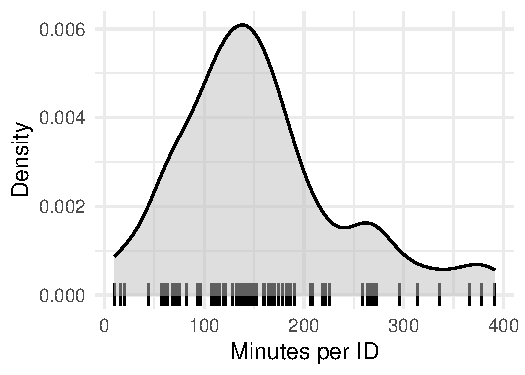
\includegraphics{Quantex_interaction_paper_files/figure-latex/quantex-minutes-per-child-1} 

}

\caption{Video recording duration (in minutes) per Child in the Quantex Dataset.}\label{fig:quantex-minutes-per-child}
\end{figure}

\subsection{Annotation Strategy}\label{annotation-strategy}

The dataset annotations cover four key elements: persons, faces, gaze direction, and objects the child interacts with. For each detected person (or reflection of a person, such as in a mirror) and face, additional attributes, such as age and gender, are collected. Gaze information indicates whether a detected person's gaze is directed toward the child or not. Faces are annotated even when occluded or blurry to ensure comprehensive coverage of interactions. Partially visible faces are also annotated if key facial features, such as the nose, eyes, or mouth, remain identifiable. Objects are annotated only when the child is actively interacting with them. These objects are categorized into six distinct groups: book, screen, animal, food, toy, and kitchenware, with an additional category for other objects. The annotation strategy is summarized in Figure \ref{fig:camera-cvat-activity-classes}.

The annotations were generated manually by a team of human annotators. Each video was randomly assigned to an initial annotator, and then reviewed by a second annotator to ensure consistency and accuracy. This peer review process helped to identify and resolve discrepancies, ensuring high-quality annotations.

\begin{figure}

{\centering 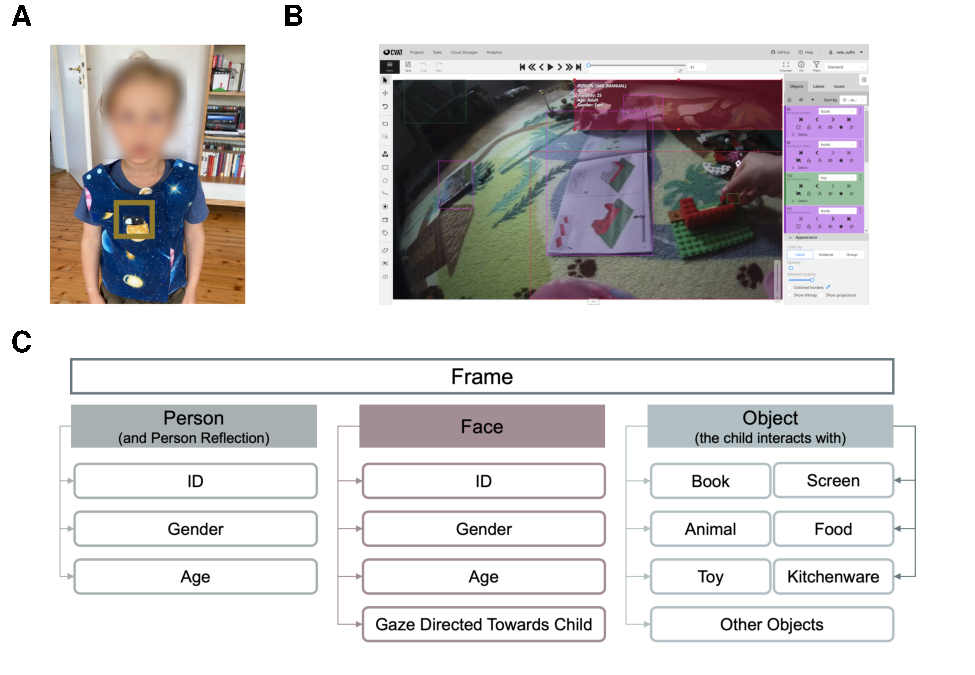
\includegraphics{Quantex_interaction_paper_files/figure-latex/camera-cvat-activity-classes-1} 

}

\caption{\textbf{A} – Vest with the embedded camera worn by the children, \textbf{B} – CVAT platform utilized for video annotation, \textbf{C} – Annotation Strategy in the Quantex dataset.}\label{fig:camera-cvat-activity-classes}
\end{figure}

\subsection{Data Preprocessing}\label{data-preprocessing}

For the video data, the annotation strategy required persons, faces, and objects to be labeled even when only partially visible, as long as key features such as facial landmarks (e.g., nose, eyes, or mouth) or parts of a person or object were clearly visible. To prepare the video data for analysis, one frame per second was annotated, corresponding to every 30th frame in the video. This frame sampling was chosen to balance the need for a representative sample of the video while keeping the analysis manageable. Similarly, every 30th raw frame was extracted from the annotated video files for further processing. No preprocessing was applied to the audio data, which was used in its raw form for analysis.

\subsection{Automated Analysis Pipeline}\label{automated-analysis-pipeline}

Our automated analysis pipeline consists of four key modules: person and face detection, gaze classification, object detection, and voice type classification. Each module operates independently, utilizing separate machine learning models. Except for the voice type classifier, all models were trained on the Quantex dataset.

The pipeline follows a sequential process:
1. Person and face detection identifies the presence of individuals in the video frames.
2. Gaze classification determines whether detected faces are looking at the child.
3. Voice type classification detects the presence of speech and identifies whether the speaker is the key child, another child, or an adult.
4. Object detection provides insights into the types of objects children interact with, both in social and independent play contexts.

By integrating these modules, our pipeline enables a comprehensive analysis of children's everyday experiences, capturing both social interactions and independent play

In the following sections, we describe each module in detail, including training data, model architecture, and evaluation metrics. A full technical analysis of each algorithm is provided in the \hyperref[supplementary-material]{Supplementary Material}.

\subsubsection{Person \& Face Detection}\label{person-face-detection}

\subsubsection{Gaze Classification}\label{gaze-classification}

\subsubsection{Object Detection}\label{object-detection}

\subsubsection{Voice Detection and Classification}\label{voice-detection-and-classification}

\section{Results}\label{results}

\subsection{Presence of Aspects of Social Interaction}\label{presence-of-aspects-of-social-interaction}

\subsubsection{Presence of a Person}\label{presence-of-a-person}

\subsubsection{Presence of a Face}\label{presence-of-a-face}

\subsubsection{Presence of Gaze}\label{presence-of-gaze}

\subsubsection{Presence of Language}\label{presence-of-language}

\subsection{Co-occurrence of Aspects of Social Interaction}\label{co-occurrence-of-aspects-of-social-interaction}

\section{General Discussion}\label{general-discussion}

\newpage

\section{References}\label{references}

\newpage

\section{Supplementary Material}\label{supplementary-material}

\subsection{Yolo11m: Person and Face Detection}\label{yolo11m-person-and-face-detection}

In our study, we utilized Ultralytics' YOLO11, the ``latest iteration in the Ultralytics YOLO series of real-time object detectors'' (Jocher \& Qiu, 2024), trained on the COCO dataset. Released in October 2024, YOLO11 introduces architectural improvements such as the C2PSA block (Convolutional Block with Parallel Spatial Attention), which enhances spatial attention within feature maps, allowing the model to focus more precisely on critical areas of an image compared to previous Yolo versions. Additionally, YOLO11 incorporates the C3K2 block, designed to be faster and more efficient, enhancing the overall performance of the feature aggregation process (Khanam \& Hussain, 2024). These advancements make the YOLO11 detection model, pretrained on COCO, well-suited for training on our egocentric dataset, which captures dynamic movements from a camera perspective on chest height.

However, our dataset presents unique challenges due to the egocentric viewpoint, as the body parts of the child wearing the camera frequently appear in the footage. To prevent misclassification, we use a dedicated annotation scheme where all individuals in the scene are labeled as ``person,'' but each is assigned a unique ID. The key child, who wears the camera, is always assigned ID = 1. During preprocessing, we map the key child (ID = 1) into a separate category, ``child body parts,'' to distinguish their presence from other individuals. Since standard YOLO models do not inherently make this distinction, we fine-tune YOLO11m to recognize and differentiate between the key child's body parts and other people. This adaptation ensures accurate person detection while minimizing false positives from the child's own body, ultimately allowing for more precise analyses of social interactions. Additionally, YOLO11 does not include a predefined ``face'' class in its standard configuration, further underscoring the need for fine-tuning to meet the specific requirements of our dataset.

\subsubsection{Dataset Splitting}\label{dataset-splitting}

We started data preprocessing with a dataset comprising a total of 113799 frames from 80 annotated videos. Prior to splitting this dataset into training, validation, and testing datasets, we analyzed the proportion of frames containing annotated persons as well as faces versus those without any annotations. Our analysis showed that at least one person was present in 45.25\% of the frames and at least one face was visible in 45.25\% of the frames. We applied a stratified split to ensure that each of the training, validation, and testing dataset preserved the original ratio of frames with persons, frames with faces to frames without any persons or faces. As a result, the final data distribution, displayed in detail in table \ref{tab:person-dataset-splits}) consisted of 91038 frames in the training dataset, 11379 frames in the validation and 11382 frames in the testing dataset, guaranteeing that the model's performance evaluation remained accurate to the real-world data distribution.

\begin{table}[tbp]

\begin{center}
\begin{threeparttable}

\caption{\label{tab:person-dataset-splits}Dataset splits for the YOLO11 person and face detection model trained on the Quantex dataset. The table shows the total number of frames, as well as the number of frames with only persons, only faces, both persons and faces, and no persons or faces in the training, validation, and testing datasets.}

\begin{tabular}{llllll}
\toprule
Quantex & \multicolumn{1}{c}{Percentage} & \multicolumn{1}{c}{Training} & \multicolumn{1}{c}{Validation} & \multicolumn{1}{c}{Testing} & \multicolumn{1}{c}{Total}\\
\midrule
Only Person(s) & 30.19 & 27484 & 3435 & 3436 & 34355\\
Only Face(s) & 0.22 & 202 & 25 & 26 & 253\\
Persons and Faces & 14.83 & 13506 & 1688 & 1689 & 16883\\
No Person or Face & 54.75 & 49846 & 6230 & 6232 & 62308\\
Total &  & 91038 & 11378 & 11573 & 113799\\
\bottomrule
\end{tabular}

\end{threeparttable}
\end{center}

\end{table}

\subsubsection{Training and Convergence}\label{training-and-convergence}

Model training was conducted on a Linux server equipped with an Intel(R) Xeon(R) Silver 4214Y CPU @ 2.20GHz with 48 cores, a Quadro RTX 8000 GPU and 188 GB of RAM. The model was trained for a total of 86 epochs, taking 200 hours to complete. Training utilized YOLO11's built-in data augmentation, an image size of 640, a batch size of 16, a cosine annealing learning rate scheduler (Loshchilov \& Hutter, 2017), and early stopping after 10 epochs without improvement, with a maximum of 200 epochs.

The loss function of the YOLO11 model comprises three main components: Box Loss, Classification Loss, and Distribution Focal Loss (DFL) (Li et al., 2020; Terven, Cordova-Esparza, Ramirez-Pedraza, Chavez-Urbiola, \& Romero-Gonzalez, 2024). \emph{Box Loss} quantifies the difference between predicted bounding boxes and ground truth boxes, ensuring precise localization of detected objects by penalizing inaccuracies in position and size. \emph{Classification Loss} evaluates the model's ability to correctly assign detected objects to their respective classes, reducing false positives and false negatives. \emph{Distribution Focal Loss} enhances the model's ability to detect challenging objects, particularly small or partially occluded ones, by refining the localization of bounding box coordinates and emphasizing hard-to-detect instances. Together, these loss components contribute to a more robust and accurate detection model.

During the training process, we observed that all three loss components decreased over time, indicating effective learning and improved performance, as visible in in figure \ref{fig:person-loss-curves}. A steady decrease in Box Loss indicates that the model is becoming increasingly accurate in localizing persons, faces and child body parts within frames. Similarly, the steady convergence of the Classification Loss reveals the model's increasing ability to reliably classifiy the detected object in either ``person'', ``face'' or ``child body part''. The decrease in DFL over time indicates that the model is getting better at focusing on and correctly identifying difficult-to-detect persons, faces or child body parts, which improves its overall detection capabilities. Conclusively, the loss curves show that the model effectively learned to localize and identify the target classes during the training period.

\begin{figure}

{\centering 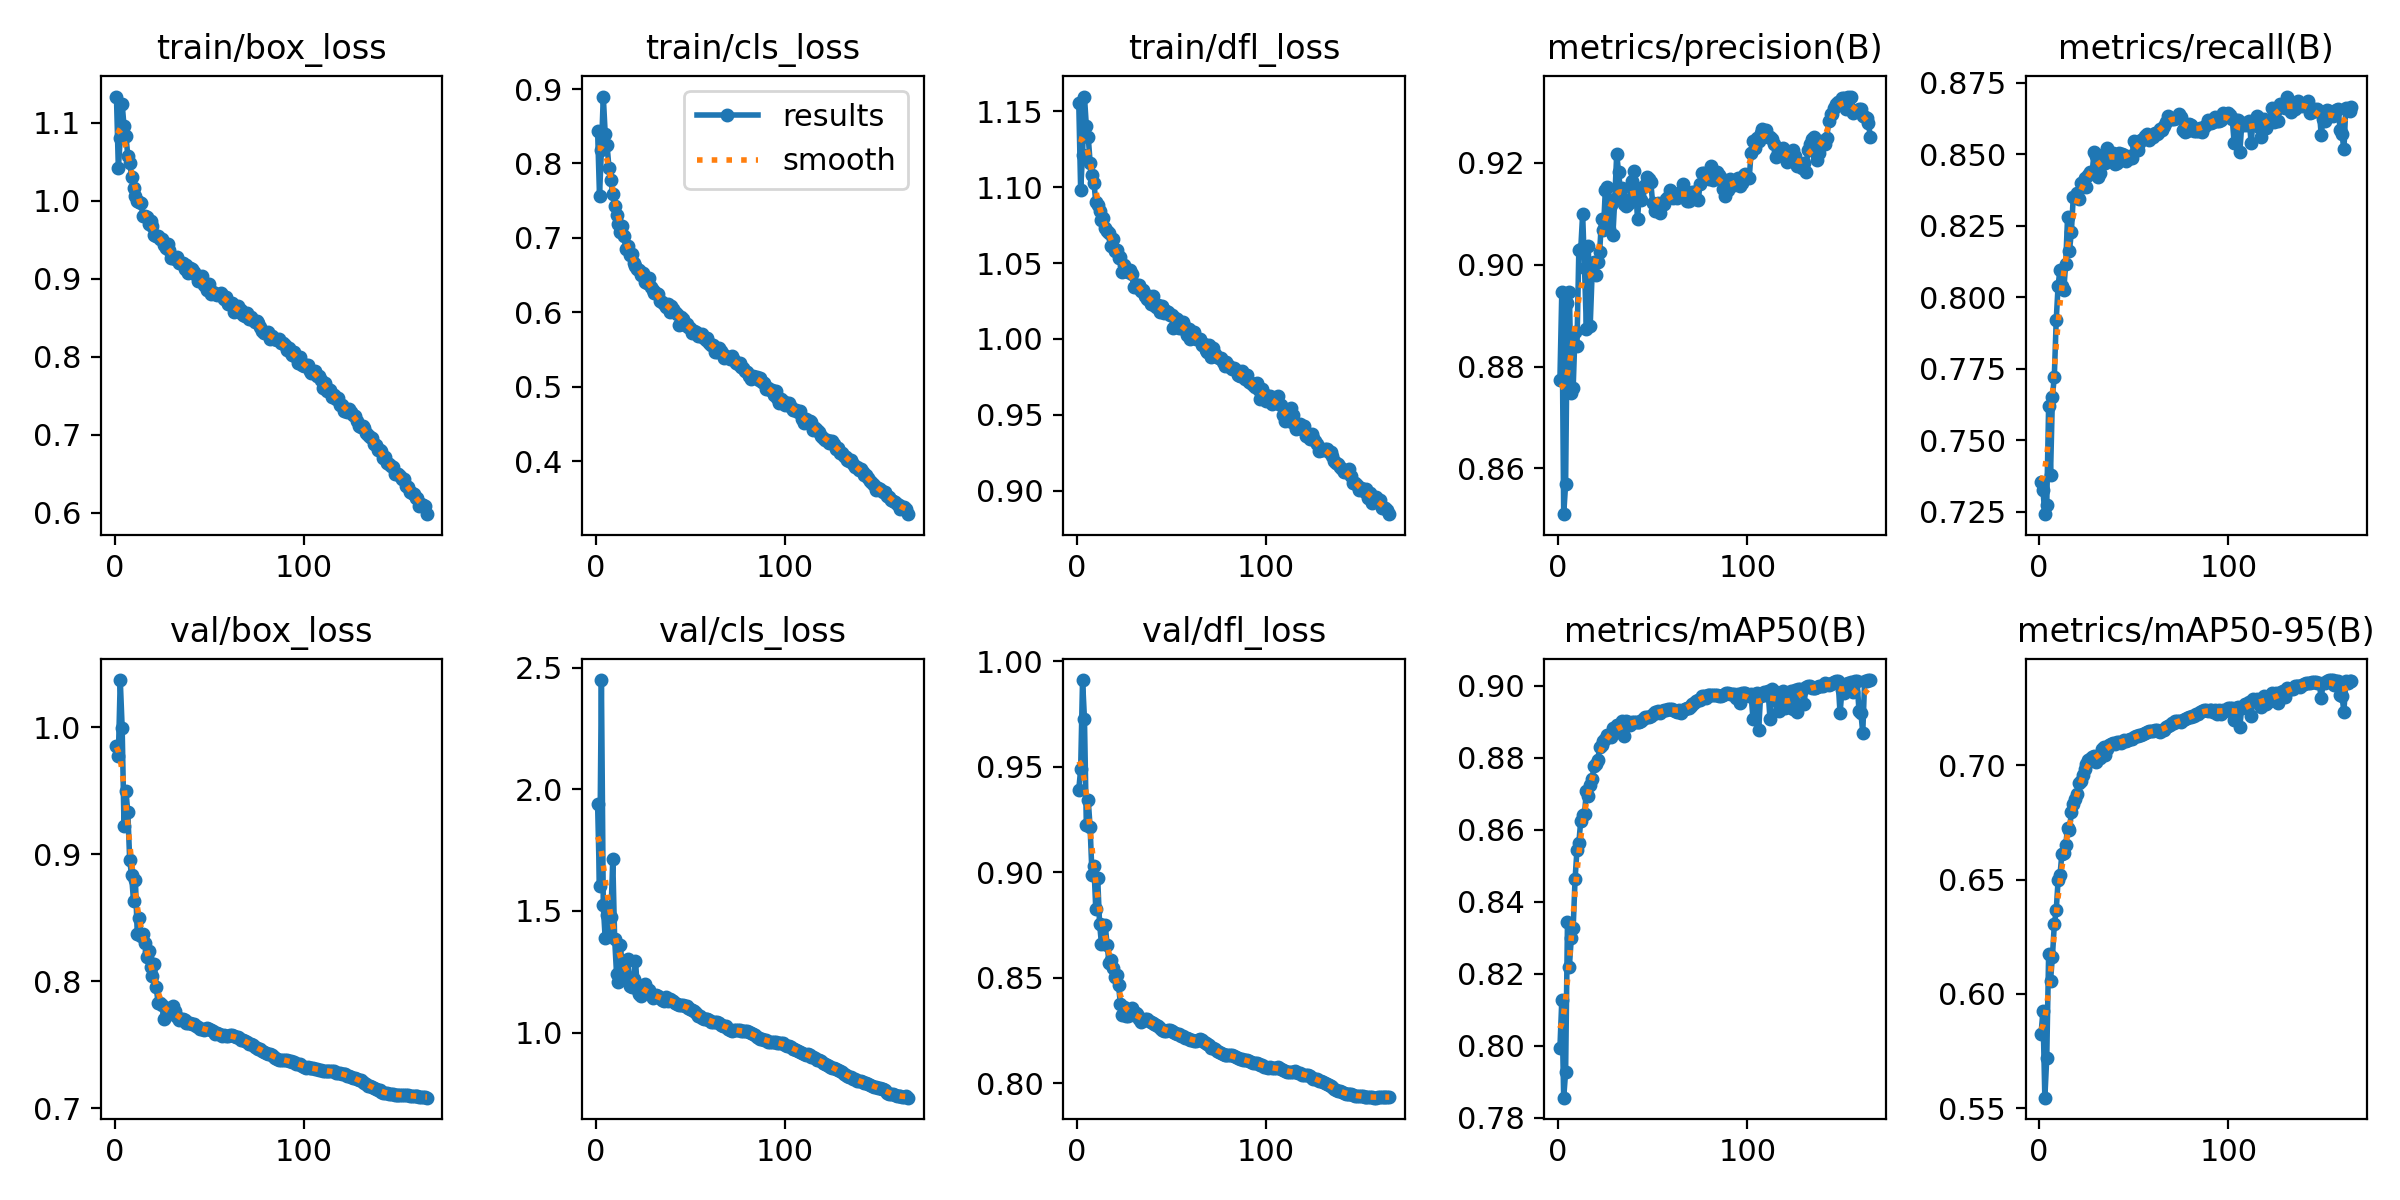
\includegraphics[width=450px]{images/yolo_face_loss_curves} 

}

\caption{Training and Validation Loss Curves for the YOLO11 person detection model.}\label{fig:person-loss-curves}
\end{figure}

\subsubsection{Model Evaluation Metrics}\label{model-evaluation-metrics}

The YOLO11 model achieved a precision of 0.92 and a recall of 0.87 on the testing set, resulting in an F1-score of 0.90. These metrics, summarized in table \ref{tab:person-detection-metrics-detailed} indicate the model's strong performance in accurately identifying faces while minimizing the number of missed detections and false positives. The precision-recall curve, displayed in figure \ref{fig:person-metrics}, further illustrates this performance, with the curve remaining close to the top-left corner. This positioning signifies that the model maintains high precision and recall across various thresholds, underscoring its effectiveness in detecting faces with confidence.

Analysis of the confusion matrix reveals that 86\% of all faces are correctly identified by the model, corresponding to 1905 true positives, while 234 faces were missed (false negatives). False negatives predominantly occurred in scenarios where faces were in the background, blurred due to motion, or occluded by the child's body. In such instances, adjacent frames often provided clearer views, aiding in more accurate classification. The model exhibited a false positive rate of approximately 2.72\%, with 251 frames incorrectly classified as containing faces when none were present. These false positives were often attributed to objects or toys resembling facial features. In face detection systems, achieving a balance between false positives and false negatives is crucial. Given this context, a 2.1\% false positive rate is generally considered acceptable.

To provide a comprehensive understanding of the model's performance, we have included visual examples of true positives, false positives, and false negatives in figure \ref{fig:person-detection-examples}. These images highlight the model's strengths and areas where challenges persist, offering insights into specific scenarios that influence detection accuracy.

Overall, the YOLO11 model demonstrates robust performance in face detection tasks. However, challenges remain in dynamic scenarios, particularly with partially visible, rotated, or side-view faces. These findings underscore the complexities inherent in analyzing egocentric video data, where movement and varying perspectives introduce additional challenges.

\begin{table}[tbp]

\begin{center}
\begin{threeparttable}

\caption{\label{tab:person-detection-metrics-detailed}Evaluation metrics for the YOLO11m detection model trained on the Quantex dataset to detect persons and faces while distinguishing between the key child and other individuals. False Positive Rate and False Negative Rate are given in percentages.}

\begin{tabular}{llllll}
\toprule
Dataset & \multicolumn{1}{c}{Precision} & \multicolumn{1}{c}{Recall} & \multicolumn{1}{c}{F1-Score} & \multicolumn{1}{c}{False Positive Rate} & \multicolumn{1}{c}{False Negative Rate}\\
\midrule
Quantex & 0 & 0 & 0 & 0 & 0\\
\bottomrule
\end{tabular}

\end{threeparttable}
\end{center}

\end{table}

\begin{figure}

{\centering 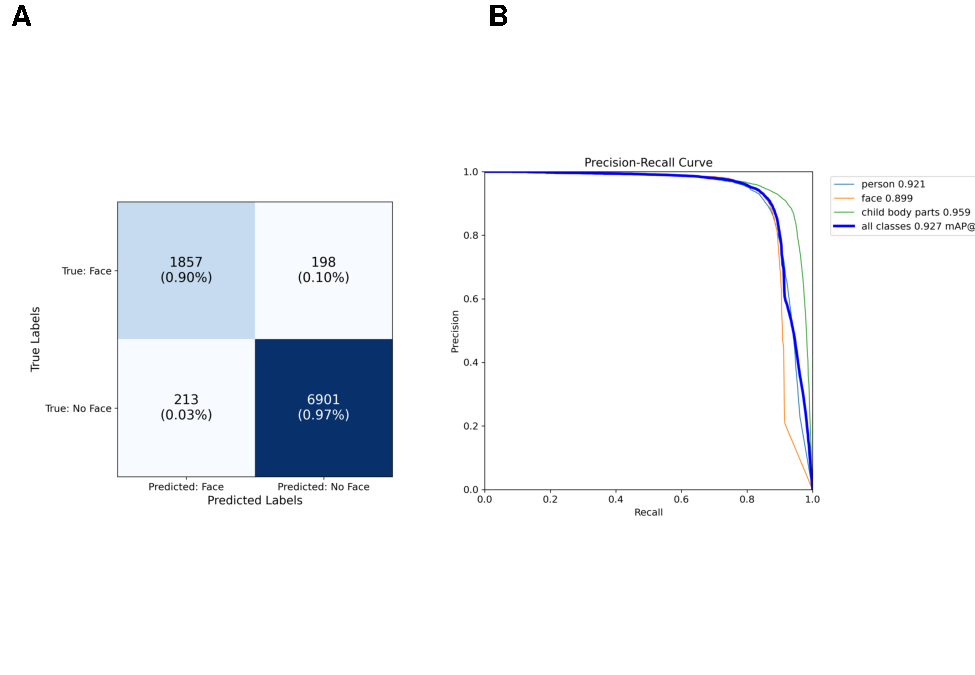
\includegraphics{Quantex_interaction_paper_files/figure-latex/person-metrics-1} 

}

\caption{\textbf{A} - Confusion Matrix for the YOLO11 person detection model trained on the Quantex dataset. \textbf{B} - Precision-Recall Curve for the YOLO11 person detection model.}\label{fig:person-metrics}
\end{figure}

\begin{figure}

{\centering \includegraphics{Quantex_interaction_paper_files/figure-latex/person-detection-examples-1} 

}

\caption{\textbf{A}, \textbf{B} - Examples of True Positives, \textbf{C}, \textbf{D} – Examples of False Negatives, \textbf{E}, \textbf{F} – Examples of False Positives in the YOLO11 person detection model.}\label{fig:person-detection-examples}
\end{figure}

\subsection{Yolo11m-cls: Gaze Classification}\label{yolo11m-cls-gaze-classification}

In the gaze classification part of our study, we employed Ultralytics' YOLO11 architecture (Jocher \& Qiu, 2024), more specifically the yolo11m classification model which is pretrained on ImageNet. The video data, collected from a camera on chest height, present unique challenges due to its egocentric perspective. This viewpoint sometimes introduced motion blur and the particular recoring angle can make it difficult to determine whether a person's gaze is directed at the child, even for human annotators. We therefore defined to classify a person's gaze as ``directed towards the child'' when the person's gaze is oriented towards the child's face, body, or in their general direction. This included cases where the person is looking directly at the camera, which is worn by the child, or slightly upward, estimating where the child's head would be. For each face, we annotated the gaze as either directed at the child (``gaze'') or not (``no gaze''). Due to the architectural enhancements of YOLO11, such as the C2PSA block, which improves the model's ability to focus on critical regions within an image, we chose YOLO11 for our gaze classification task and fine-tuned the pretrained Yolo11m model to classify gaze accordingly.

\subsubsection{Dataset Splitting}\label{dataset-splitting-1}

For the gaze classification task, we utilized a subset of the Quantex dataset, focusing specifically on frames containing annotated faces. This subset comprised the cut-out faces extracted from the annotated face bounding boxes, resulting in 20889 frames from 64 annotated videos. An analysis of each annotated face's gaze property revealed that 21.25\% of the faces were annotated as having gaze directed towards the child. Although the dataset is imbalanced, with ``no gaze'' as the majority class, we decided not to balance it, as too much data would have been lost, and the resulting dataset would have been too small. To preserve the existing gaze-to-no-gaze ratio, we instead employed a stratified sampling technique, ensuring proportional representation across the training, validation, and testing datasets. This approach resulted in the data distribution presented in Table (\textbf{ref?})(tab:gaze-dataset-splits). Specifically, the training set comprised 16710 frames, the validation set 2088 frames, and the testing set 2091 frames. By maintaining consistent class distribution across all subsets, we aimed to ensure that the model's performance evaluation accurately reflects real-world data distributions.

\begin{table}[tbp]

\begin{center}
\begin{threeparttable}

\caption{\label{tab:gaze-dataset-splits}Dataset splits for the YOLO11 gaze classification model trained on the Quantex dataset. The table shows the total number of frames, as well as the number of frames with gaze and no gaze in the training, validation, and testing datasets. 'Gaze' indicates frames where the person's gaze is directed towards the child, while 'No Gaze' indicates frames where the person's gaze is not directed towards the child. Ratios are given in percentages.}

\begin{tabular}{llllll}
\toprule
Quantex & \multicolumn{1}{c}{Ratio} & \multicolumn{1}{c}{Training} & \multicolumn{1}{c}{Validation} & \multicolumn{1}{c}{Testing} & \multicolumn{1}{c}{Total}\\
\midrule
Gaze & 21.25 & 3550 & 443 & 445 & 4438\\
No Gaze & 78.75 & 13160 & 1645 & 1646 & 16451\\
Total & 100.00 & 16710 & 2088 & 2091 & 20889\\
\bottomrule
\end{tabular}

\end{threeparttable}
\end{center}

\end{table}

\subsubsection{Training and Convergence}\label{training-and-convergence-1}

We trained the gaze classification model on the same linux server that was used for the person and face detection model training. The model was trained for a total of 165 epochs, taking 283 hours to complete. Similar to the person and face detection model, model training was conducted applying an image size of 640, a batch size of 16, a cosine annealing learning rate scheduler (Loshchilov \& Hutter, 2017), and early stopping after 10 epochs without improvement, with a maximum of 200 epochs.

Figure \ref{fig:person-loss-curves} provides an overview of the loss curves for the gaze classification model, showing the Box Loss, Classification Loss, and Distribution Focal Loss (DFL) over the training period.
- tbd

\subsubsection{Model Evaluation Metrics}\label{model-evaluation-metrics-1}

\subsection{Object Detection}\label{object-detection-1}

\subsection{Voice Type Classification}\label{voice-type-classification}

Regarding the audio component of our interaction analysis, we aimed to use a model that not only detects the presence of speech but also distinguishes between the key child wearing the camera and other speakers. This distinction is crucial for understanding the dynamics of the interactions and the role of the key child in the social context. To achieve this, we applied the Voice Type Classifier (Lavechin, Bousbib, Bredin, Dupoux, \& Cristia, 2020), an open-source model designed to identify five different voice types: key child, other child, female adult, male adult, and speech in general. The model is based on a convolutional neural network (CNN) architecture and was trained on 260 hours of child-centered recordings across 10 different languages.

Although the Quantex dataset does not include explicit audio labels, we are confident in the model's suitability for our data. Prior testing on a similar labeled dataset which was also collected in our lab, ChildLens, demonstrated that the Voice Type Classifier achieved an F1 score of 58.1 (reference to ChildLens paper), which is comparable to the F1 score of 57.3 reported on the original training dataset. These results indicate that the model generalizes well to child-centered recordings, making it a reliable choice for our analysis.

We applied the Voice Type Classifier to the extracted audio data from the Quantex dataset using the code provided by the authors of the voice type classifier (Lavechin, 2020). The model was used to detect the presence of speech and classify the speaker into one of the five predefined categories.

\newpage

\section{References}\label{references-1}

\begingroup
\setlength{\parindent}{-0.5in}
\setlength{\leftskip}{0.5in}

\phantomsection\label{refs}
\begin{CSLReferences}{1}{0}
\bibitem[\citeproctext]{ref-baevskiWav2vec20Framework2020}
Baevski, A., Zhou, H., Mohamed, A., \& Auli, M. (2020). Wav2vec 2.0: {A Framework} for {Self-Supervised Learning} of {Speech Representations}. \url{https://doi.org/10.48550/ARXIV.2006.11477}

\bibitem[\citeproctext]{ref-bergelsonEverydayLanguageInput2023}
Bergelson, E., Soderstrom, M., Schwarz, I.-C., Rowland, C. F., Ramírez-Esparza, N., R. Hamrick, L., \ldots{} Cristia, A. (2023). Everyday language input and production in 1,001 children from six continents. \emph{Proceedings of the National Academy of Sciences}, \emph{120}(52), e2300671120. \url{https://doi.org/10.1073/pnas.2300671120}

\bibitem[\citeproctext]{ref-caoOpenPoseRealtimeMultiPerson2018}
Cao, Z., Hidalgo, G., Simon, T., Wei, S.-E., \& Sheikh, Y. (2018). {OpenPose}: {Realtime Multi-Person 2D Pose Estimation} using {Part Affinity Fields}. \url{https://doi.org/10.48550/ARXIV.1812.08008}

\bibitem[\citeproctext]{ref-carpendaleWhatMakesUs2020}
Carpendale, J., \& Lewis, C. (2020). \emph{What {Makes Us Human}: {How Minds Develop} through {Social Interactions}} (1st ed.). Routledge. \url{https://doi.org/10.4324/9781003125105}

\bibitem[\citeproctext]{ref-carreiraQuoVadisAction2017}
Carreira, J., \& Zisserman, A. (2017). Quo {Vadis}, {Action Recognition}? {A New Model} and the {Kinetics Dataset}. \url{https://doi.org/10.48550/ARXIV.1705.07750}

\bibitem[\citeproctext]{ref-chenDyadicAffectParentChild2023}
Chen, H., Alghowinem, S., Jang, S. J., Breazeal, C., \& Park, H. W. (2023). Dyadic {Affect} in {Parent-Child Multimodal Interaction}: {Introducing} the {DAMI-P2C Dataset} and its {Preliminary Analysis}. \emph{IEEE Transactions on Affective Computing}, \emph{14}(4), 3345--3361. \url{https://doi.org/10.1109/TAFFC.2022.3178689}

\bibitem[\citeproctext]{ref-debarbaroTenLessonsInfants2022}
De Barbaro, K., \& Fausey, C. M. (2022). Ten {Lessons About Infants}' {Everyday Experiences}. \emph{Current Directions in Psychological Science}, \emph{31}(1), 28--33. \url{https://doi.org/10.1177/09637214211059536}

\bibitem[\citeproctext]{ref-donnellyLongitudinalRelationshipConversational2021}
Donnelly, S., \& Kidd, E. (2021). The {Longitudinal Relationship Between Conversational Turn}‐{Taking} and {Vocabulary Growth} in {Early Language Development}. \emph{Child Development}, \emph{92}(2), 609--625. \url{https://doi.org/10.1111/cdev.13511}

\bibitem[\citeproctext]{ref-fraileUpStoryUppsalaStorytelling2024}
Fraile, M., Calvo-Barajas, N., Apeiron, A. S., Varni, G., Lindblad, J., Sladoje, N., \& Castellano, G. (2024). {UpStory}: The {Uppsala Storytelling} dataset. \url{https://doi.org/10.48550/ARXIV.2407.04352}

\bibitem[\citeproctext]{ref-heyesCognitiveGadgetsCultural2018}
Heyes, C. M. (2018). \emph{Cognitive gadgets: The cultural evolution of thinking}. Cambridge (Mass.): Harvard University press.

\bibitem[\citeproctext]{ref-jocherUltralyticsYOLO112024}
Jocher, G., \& Qiu, J. (2024). \emph{Ultralytics {YOLO11}}. Retrieved from \url{https://github.com/ultralytics/ultralytics}

\bibitem[\citeproctext]{ref-khanamYOLOv11OverviewKey2024}
Khanam, R., \& Hussain, M. (2024, October 23). {YOLOv11}: {An Overview} of the {Key Architectural Enhancements}. \url{https://doi.org/10.48550/arXiv.2410.17725}

\bibitem[\citeproctext]{ref-lavechinVoiceTypeClassifier2020}
Lavechin, M. (2020). \emph{Voice {Type Classifier}}. Retrieved from \url{https://github.com/MarvinLvn/voice-type-classifier}

\bibitem[\citeproctext]{ref-lavechinOpensourceVoiceType2020}
Lavechin, M., Bousbib, R., Bredin, H., Dupoux, E., \& Cristia, A. (2020). An open-source voice type classifier for child-centered daylong recordings. \url{https://doi.org/10.48550/ARXIV.2005.12656}

\bibitem[\citeproctext]{ref-liGeneralizedFocalLoss2020}
Li, X., Wang, W., Wu, L., Chen, S., Hu, X., Li, J., \ldots{} Yang, J. (2020, June 8). Generalized {Focal Loss}: {Learning Qualified} and {Distributed Bounding Boxes} for {Dense Object Detection}. \url{https://doi.org/10.48550/arXiv.2006.04388}

\bibitem[\citeproctext]{ref-longBabyViewDatasetHighresolution2024}
Long, B., Xiang, V., Stojanov, S., Sparks, R. Z., Yin, Z., Keene, G. E., \ldots{} Frank, M. C. (2024, June 14). The {BabyView} dataset: {High-resolution} egocentric videos of infants' and young children's everyday experiences. \url{https://doi.org/10.48550/arXiv.2406.10447}

\bibitem[\citeproctext]{ref-loshchilovSGDRStochasticGradient2017}
Loshchilov, I., \& Hutter, F. (2017, May 3). {SGDR}: {Stochastic Gradient Descent} with {Warm Restarts}. \url{https://doi.org/10.48550/arXiv.1608.03983}

\bibitem[\citeproctext]{ref-piagetPartCognitiveDevelopment1964}
Piaget, J. (1964). Part {I}: {Cognitive} development in children: {Piaget} development and learning. \emph{Journal of Research in Science Teaching}, \emph{2}(3), 176--186. \url{https://doi.org/10.1002/tea.3660020306}

\bibitem[\citeproctext]{ref-redmonYouOnlyLook2015}
Redmon, J., Divvala, S., Girshick, R., \& Farhadi, A. (2015). You {Only Look Once}: {Unified}, {Real-Time Object Detection}. \url{https://doi.org/10.48550/ARXIV.1506.02640}

\bibitem[\citeproctext]{ref-rehgDecodingChildrensSocial2013}
Rehg, J. M., Abowd, G. D., Rozga, A., Romero, M., Clements, M. A., Sclaroff, S., \ldots{} Ye, Z. (2013). Decoding {Children}'s {Social Behavior}. \emph{2013 {IEEE Conference} on {Computer Vision} and {Pattern Recognition}}, 3414--3421. Portland, OR, USA: IEEE. \url{https://doi.org/10.1109/CVPR.2013.438}

\bibitem[\citeproctext]{ref-rogoffImportanceUnderstandingChildrens2018}
Rogoff, B., Dahl, A., \& Callanan, M. (2018). The importance of understanding children's lived experience. \emph{Developmental Review}, \emph{50}, 5--15. \url{https://doi.org/10.1016/j.dr.2018.05.006}

\bibitem[\citeproctext]{ref-roweDifferencesEarlyGesture2009}
Rowe, M. L., \& Goldin-Meadow, S. (2009). Differences in {Early Gesture Explain SES Disparities} in {Child Vocabulary Size} at {School Entry}. \emph{Science}, \emph{323}(5916), 951--953. \url{https://doi.org/10.1126/science.1167025}

\bibitem[\citeproctext]{ref-royPredictingBirthSpoken2015}
Roy, B. C., Frank, M. C., DeCamp, P., Miller, M., \& Roy, D. (2015). Predicting the birth of a spoken word. \emph{Proceedings of the National Academy of Sciences}, \emph{112}(41), 12663--12668. \url{https://doi.org/10.1073/pnas.1419773112}

\bibitem[\citeproctext]{ref-ruffmanExposureBehavioralRegularities2023}
Ruffman, T., Chen, L., Lorimer, B., Vanier, S., Edgar, K., Scarf, D., \& Taumoepeau, M. (2023). Exposure to behavioral regularities in everyday life predicts infants' acquisition of mental state vocabulary. \emph{Developmental Science}, \emph{26}(4), e13343. \url{https://doi.org/10.1111/desc.13343}

\bibitem[\citeproctext]{ref-russakovskyImageNetLargeScale2014}
Russakovsky, O., Deng, J., Su, H., Krause, J., Satheesh, S., Ma, S., \ldots{} Fei-Fei, L. (2014). {ImageNet Large Scale Visual Recognition Challenge}. \url{https://doi.org/10.48550/ARXIV.1409.0575}

\bibitem[\citeproctext]{ref-smithDevelopingInfantCreates2018}
Smith, L. B., Jayaraman, S., Clerkin, E., \& Yu, C. (2018). The {Developing Infant Creates} a {Curriculum} for {Statistical Learning}. \emph{Trends in Cognitive Sciences}, \emph{22}(4), 325--336. \url{https://doi.org/10.1016/j.tics.2018.02.004}

\bibitem[\citeproctext]{ref-spanglerToddlersEverydayExperiences1989}
Spangler, G. (1989). Toddlers' {Everyday Experiences} as {Related} to {Preceding Mental} and {Emotional Disposition} and {Their Relationship} to {Subsequent Mental} and {Motivational Development}: {A Short-Term Longitudinal Study}. \emph{International Journal of Behavioral Development}, \emph{12}(3), 285--303. \url{https://doi.org/10.1177/016502548901200301}

\bibitem[\citeproctext]{ref-sullivanSAYCamLargeLongitudinal2021}
Sullivan, J., Mei, M., Perfors, A., Wojcik, E., \& Frank, M. C. (2021). {SAYCam}: {A Large}, {Longitudinal Audiovisual Dataset Recorded From} the {Infant}'s {Perspective}. \emph{Open Mind}, \emph{5}, 20--29. \url{https://doi.org/10.1162/opmi_a_00039}

\bibitem[\citeproctext]{ref-tervenLossFunctionsMetrics2024}
Terven, J., Cordova-Esparza, D. M., Ramirez-Pedraza, A., Chavez-Urbiola, E. A., \& Romero-Gonzalez, J. A. (2024, October 12). Loss {Functions} and {Metrics} in {Deep Learning}. \url{https://doi.org/10.48550/arXiv.2307.02694}

\bibitem[\citeproctext]{ref-tomaselloCulturalOriginsHuman2009}
Tomasello, M. (2009). \emph{Cultural {Origins} of {Human Cognition}}. Cambridge: Harvard University Press.

\bibitem[\citeproctext]{ref-vygotskyMindSocietyDevelopment1978}
Vygotsky, L. S. (1978). \emph{Mind in {Society}: {The Development} of {Higher Psychological Processes}}. Cambridge, MA: Harvard University Press.

\end{CSLReferences}

\endgroup

\newpage

\section{Appendix}\label{appendix}


\end{document}
